\section{Theory} \label{sec:theory}
Mass-spectrometers are used to measure the amounts of different compounds in a gas. The gas is first ionized and then the different compounds are split up according to their charge-to-mass ratio. In this experiment we used a quadrupol-mass-spectrometer.

\subsection{Working principle}
    The gaseous probe is first ionized. This is done by electrons that are detached from a glowing filament and accelerated by an electric field. They then hit the compounds of the probe.  The newly generated ions are then also accelerated by the electric field and guided through a electrodynamic quadrupole field. The three components \eqref{eq:quadstatic} of the equations of motion are given in the manual \cite{manual}.
    \begin{equation}
        \begin{aligned}
            \ddot x + \left(\frac{q}{mr_0^2}\right)\Phi_0\cdot x= 0 \\
            \ddot y - \left(\frac{q}{mr_0^2}\right)\Phi_0\cdot y= 0 \\
            \ddot z = 0 
            \label{eq:quadstatic}
        \end{aligned}
    \end{equation}
    We see that the ions will move uniformly in the $z$ direction (along the electric field) but will follow a sinusoidal path in the $xz$-plane and an exponential path in the $yz$-plane which will direct them into the walls. To mitigate this problem we will also apply an alternating voltage, this will give us the following equations of motion \eqref{eq:quadalt}:
    \begin{equation}
        \begin{aligned}
            \ddot x + \left(\frac{q}{mr_0^2}\right)(U-V\cos(\omega t))\cdot x= 0 \\
            \ddot y - \left(\frac{q}{mr_0^2}\right)(U-V\cos(\omega t))\cdot y= 0 \\
            \ddot z = 0 
            \label{eq:quadalt}
        \end{aligned}
    \end{equation}
    where $U$ is the DC-offset and $V$ the amplitude of the alternating voltage.
    The $y$-axis will act as a low-pass and the $x$-axis as a high pass, together they form a bandpass filter that only lets certain charge-to-mass ratios pass through to the detector. By adjusting the DC-offset and the alternating voltage amplitude we are able to create a stable path, that lets just one component pass through. The parameters $a$ and $q$ \eqref{eq:params} are defined in the manual \cite{manual}.
    \begin{equation}
        \begin{aligned}
            a = \frac{4eU}{m\omega^2r_0^2} \\
            q = \frac{2eV}{m\omega^2r_0^2}
            \label{eq:params}
        \end{aligned}
    \end{equation}
    The parameter $v=a/q=2U/V$ is independent of the charge-to-mass ratio and is describes the slope in the parameter space as shown in figure \ref{fig:paramspace}.
    \begin{figure}[h!]
    \centering
    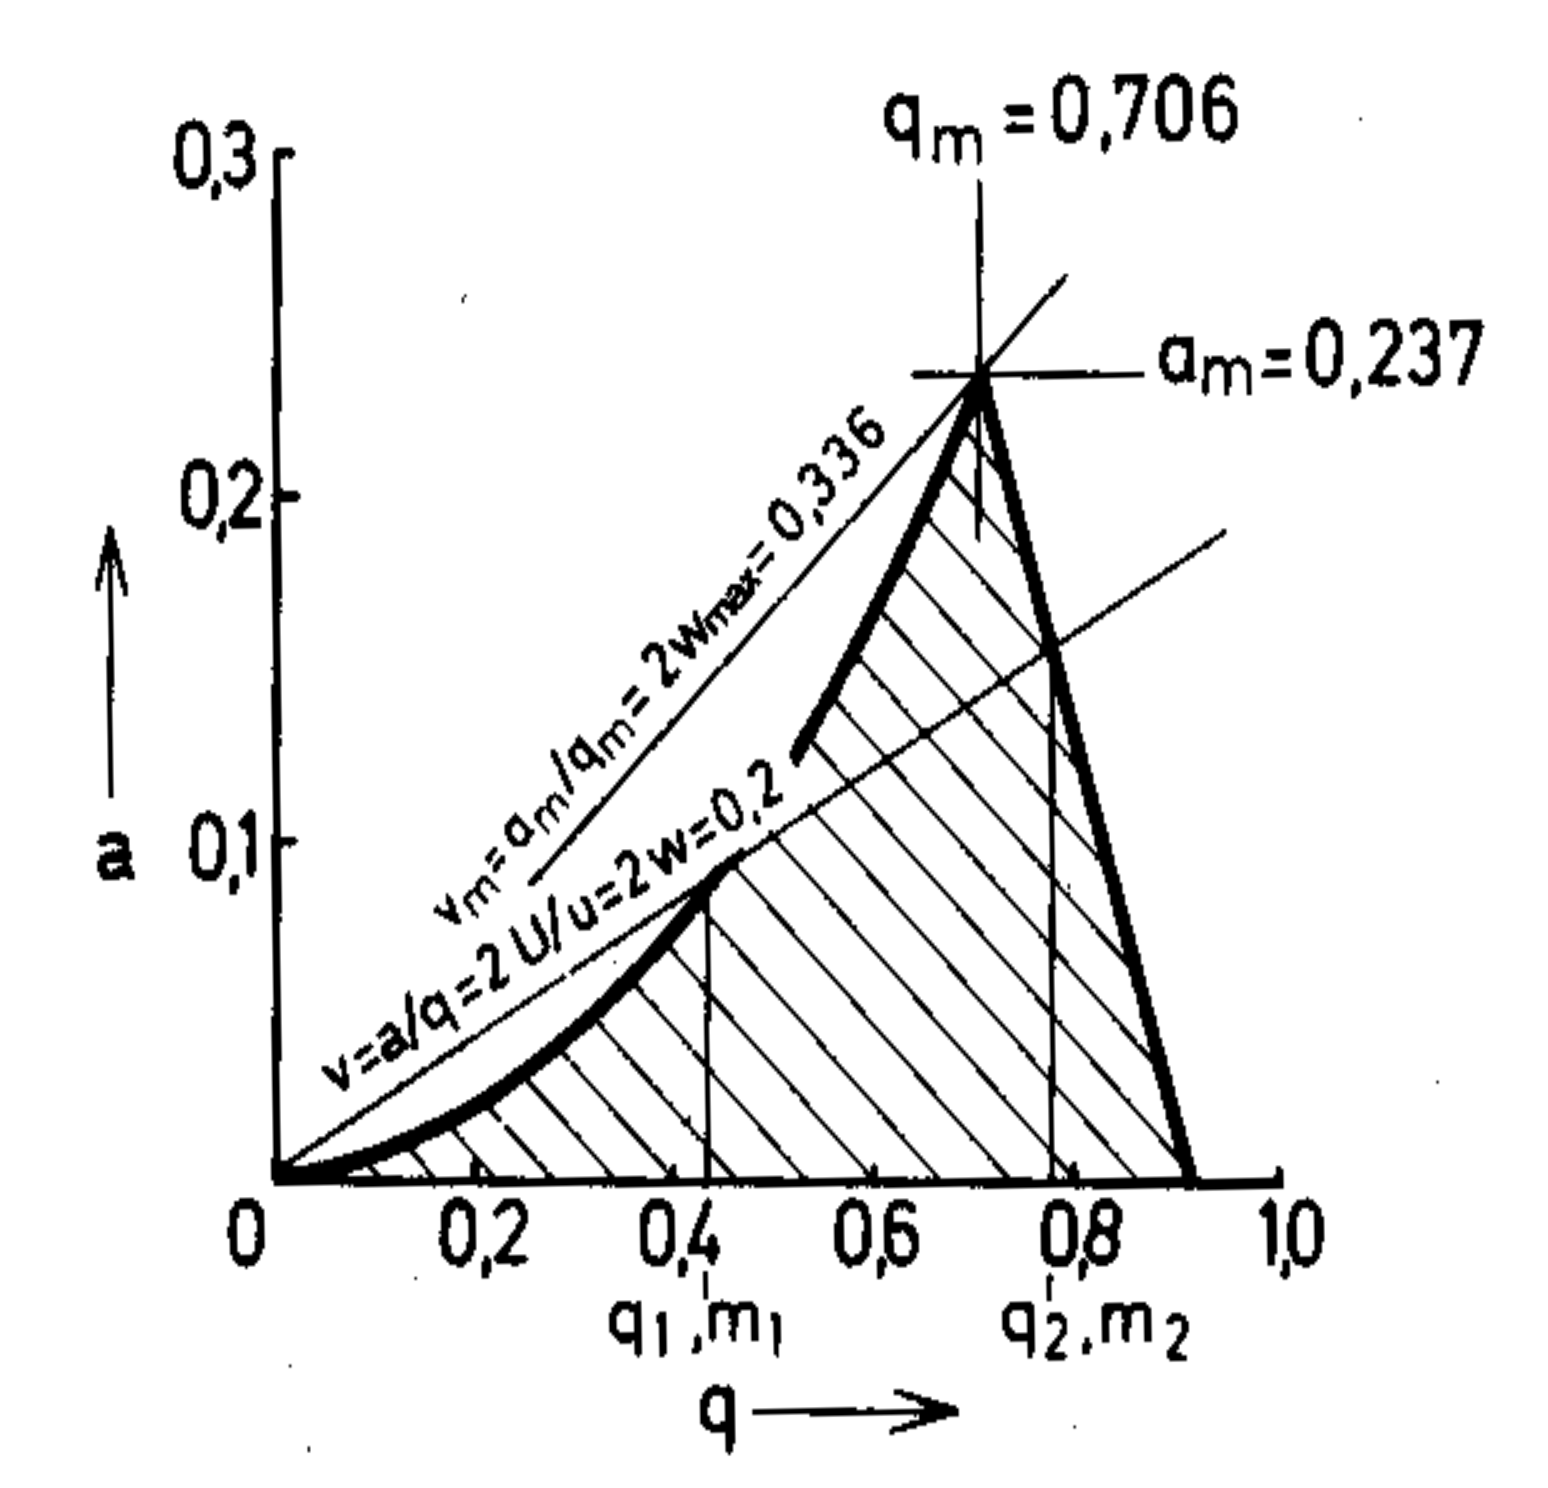
\includegraphics[width=0.5\textwidth]{Report/pictures/paramspace.png}
    \caption{The parameter space described by $a$ and $q$. \cite{manual}}
    \label{fig:paramspace}
    \end{figure}
    
    % write something about resolution and delta m
    
    
    \subsection{Detectors}
    \subsubsection{{\scshape Faraday} Detector}
    
    \subsubsection{Secondary Electron Multiplier (SEM)}